\section{tasks::sumbias Class Reference}
\label{classtasks_1_1sumbias}\index{tasks::sumbias@{tasks::sumbias}}
Inheritance diagram for tasks::sumbias::\begin{figure}[H]
\begin{center}
\leavevmode
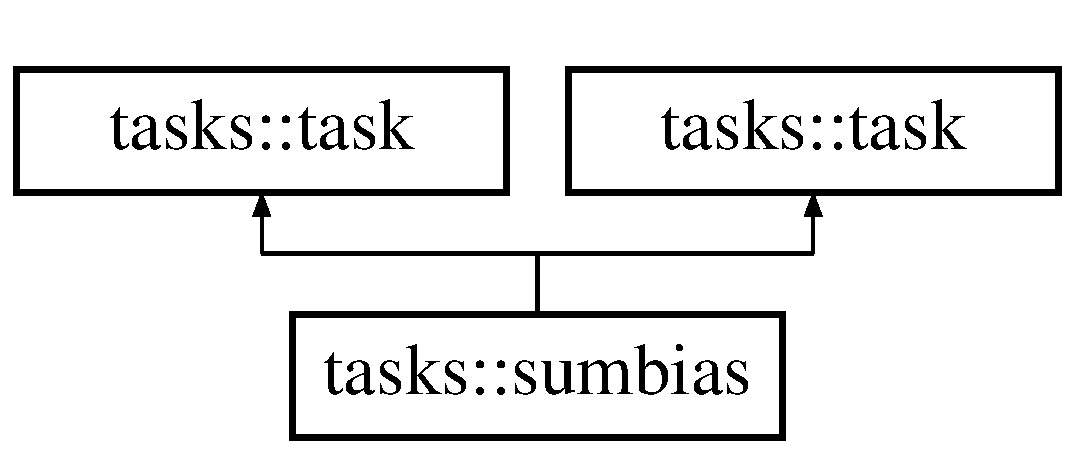
\includegraphics[height=2cm]{classtasks_1_1sumbias}
\end{center}
\end{figure}
\subsection*{Public Member Functions}
\begin{CompactItemize}
\item 
def \textbf{run}\label{classtasks_1_1sumbias_327f40e3c4132a7e7023ad778c4fad4f}

\item 
def \textbf{run}\label{classtasks_1_1sumbias_327f40e3c4132a7e7023ad778c4fad4f}

\end{CompactItemize}
\subsection*{Static Public Attributes}
\begin{CompactItemize}
\item 
string \textbf{name} = '{\bfsumbias}'\label{classtasks_1_1sumbias_b1ea35d5272e1b4c8ca78c75707b224d}

\item 
string \textbf{button\-Text} = 'Create combined BIAS'\label{classtasks_1_1sumbias_a12ef6ed5cd1e2b23f95e6df40135e0b}

\end{CompactItemize}


\subsection{Detailed Description}


\footnotesize\begin{verbatim}Combine a set of BIAS frames into the combined BIAS frame. The currently
   implemented method is median filtering of the images.
\end{verbatim}
\normalsize
 



The documentation for this class was generated from the following files:\begin{CompactItemize}
\item 
old/PANICtool-1.0/tasks.py\item 
old/tasks.py\end{CompactItemize}
